%%%%%%%%%%%%%%%%%%%%%%%%%%%%%%%%%%%%%%%%%%%%%%%%%%%%%%%%%%%%%%%%%%%%%
%% This is a (brief) model paper using the achemso class
%% The document class accepts keyval options, which should include
%% the target journal and optionally the manuscript type. 
%%%%%%%%%%%%%%%%%%%%%%%%%%%%%%%%%%%%%%%%%%%%%%%%%%%%%%%%%%%%%%%%%%%%%
\documentclass[journal=aesccq,manuscript=article,layout=twocolumn]{achemso}
\usepackage{amsmath}
\usepackage{placeins}
\usepackage{comment}
\usepackage{amssymb}
\usepackage{ulem}
\usepackage{subfig}
\usepackage{booktabs}
\usepackage{xcolor}
\definecolor{claudecoral}{HTML}{D97757}
\definecolor{codexblue}{HTML}{1F5FBF}


%%%%%%%%%%%%%%%%%%%%%%%%%%%%%%%%%%%%%%%%%%%%%%%%%%%%%%%%%%%%%%%%%%%%%
%% Place any additional packages needed here.  Only include packages
%% which are essential, to avoid problems later. Do NOT use any
%% packages which require e-TeX (for example etoolbox): the e-TeX
%% extensions are not currently available on the ACS conversion
%% servers.
%%%%%%%%%%%%%%%%%%%%%%%%%%%%%%%%%%%%%%%%%%%%%%%%%%%%%%%%%%%%%%%%%%%%%
\usepackage[version=3]{mhchem} % Formula subscripts using \ce{}
\usepackage{tikz} % For legend line drawings


%%%%%%%%%%
% Line stlye defs for Reaction Contribution Plots legend
%%%%%%%%%%

%\newcommand{\tikzSolidLine}[]{\tikz[baseline=-.7ex]{\draw[thick, solid](0,0)--(1,0);}}

\newcommand{\tikzSolidLine}{
    \begin{tikzpicture}[baseline={([yshift=-.6ex]current bounding box.center)}]    
      \draw[thick, solid] (0,0) -- (1,0);
    \end{tikzpicture}{}
}

\newcommand{\tikzDottedLine}{
    \begin{tikzpicture}[baseline={([yshift=-.6ex]current bounding box.center)}]        
      \draw[thick, dotted] (0,0) -- (1,0);
    \end{tikzpicture}{}
}

\newcommand{\tikzDashedLine}{
    \begin{tikzpicture}[baseline={([yshift=-.6ex]current bounding box.center)}]       
      \draw[thick, dashed] (0,0) -- (1,0);
    \end{tikzpicture}{}
}

\newcommand{\tikzDashDottedLine}{
    \begin{tikzpicture}[baseline={([yshift=-.6ex]current bounding box.center)}]       
      \draw[thick, dashdotted] (0,0) -- (1,0);
    \end{tikzpicture}{}
}

\newcommand{\tikzDashThreeDottedLine}{
    \begin{tikzpicture}[dash pattern=on 3pt off 2pt on 1pt off 2pt on 1pt off 2pt on 1pt off 2pt,baseline={([yshift=-.6ex]current bounding box.center)}]      
      \draw[thick] (0,0) -- (1,0);
    \end{tikzpicture}{}
}

\setcounter{secnumdepth}{4} % For /paragraph{} numbering 

\usepackage{caption}    % For subfigures
\usepackage{subcaption} % For subfigures


%%%%%%%%%%%%%%%%%%%%%%%%%%%%%%%%%%%%%%%%%%%%%%%%%%%%%%%%%%%%%%%%%%%%%
%% If issues arise when submitting your manuscript, you may want to
%% un-comment the next line.  This provides information on the
%% version of every file you have used.
%%%%%%%%%%%%%%%%%%%%%%%%%%%%%%%%%%%%%%%%%%%%%%%%%%%%%%%%%%%%%%%%%%%%%
%%\listfiles

%%%%%%%%%%%%%%%%%%%%%%%%%%%%%%%%%%%%%%%%%%%%%%%%%%%%%%%%%%%%%%%%%%%%%
%% Place any additional macros here.  Please use \newcommand* where
%% possible, and avoid layout-changing macros (which are not used
%% when typesetting).
%%%%%%%%%%%%%%%%%%%%%%%%%%%%%%%%%%%%%%%%%%%%%%%%%%%%%%%%%%%%%%%%%%%%%
\newcommand*\mycommand[1]{\texttt{\emph{#1}}}
\DeclareRobustCommand{\cb}[1]{\textbf{\textcolor{codexblue}{#1}}}

%Reaction counter for photoprocesses
\newcounter{pcounter}
\newcommand{\pcount}[1]{\refstepcounter{pcounter}\label{#1}\ref{#1}}
\renewcommand\thepcounter{P\arabic{pcounter}}

%Reaction counter for reactions
\newcounter{ncounter}
\newcommand{\ncount}[1]{\refstepcounter{ncounter}\label{#1}\ref{#1}}
\renewcommand\thencounter{N\arabic{ncounter}}


%%%%%%%%%%%%%%%%%%%%%%%%%%%%%%%%%%%%%%%%%%%%%%%%%%%%%%%%%%%%%%%%%%%%%
%% Meta-data block
%% ---------------
%% Each author should be given as a separate \author command.
%%
%% Corresponding authors should have an e-mail given after the author
%% name as an \email command. Phone and fax numbers can be given
%% using \phone and \fax, respectively; this information is optional.
%%
%% The affiliation of authors is given after the authors; each
%% \affiliation command applies to all preceding authors not already
%% assigned an affiliation.
%%
%% The affiliation takes an option argument for the short name.  This
%% will typically be something like "University of Somewhere".
%%
%% The \altaffiliation macro should be used for new address, etc.
%% On the other hand, \alsoaffiliation is used on a per author basis
%% when authors are associated with multiple institutions.
%%%%%%%%%%%%%%%%%%%%%%%%%%%%%%%%%%%%%%%%%%%%%%%%%%%%%%%%%%%%%%%%%%%%%
\author{Kristen Darnell}
\affiliation[San Jose State University]{Department of Astronomy, San Jose State University, San Jose, California, USA}
\author{Daniel Lopez-Sanders}
\affiliation[Benedictine College]{Department of Physics and Astronomy, Benedictine College, Atchison, KS, USA}
\author{Deaton Warren}
\affiliation[VMI]{Department of Chemistry, Virginia Military Institute, Lexington, VA 24450 USA}
\author{River-Allen Carroll}
\affiliation[VMI]{Department of Chemistry, Virginia Military Institute, Lexington, VA 24450 USA}
\author{Emma Stanley}
\affiliation[VMI]{Department of Chemistry, Virginia Military Institute, Lexington, VA 24450 USA}
\author{Liton Majumdar}
\affiliation[IIS]{Exoplanets and Planetary Formation Group, School of Earth and Planetary Sciences, National Institute of Science Education and Research, Jatni 752050, Odisha, India}
\alsoaffiliation[HB]{Homi Bhabha National Institute, Training School Complex, Anushaktinagar, Mumbai 400094, India}
\author{Paola Caselli}
\affiliation[MPE]{Center for Astrochemical Studies, Max Planck Institute for Extraterrestrial Physics, Garching, 85741 Germany}
\author{Christopher Arumainayagam}
\affiliation[Wellesley]{Department of Chemistry, Wellesley College, Wellesley, 02481 MA}
\author{Christopher N. Shingledecker}
\affiliation[VMI]{Department of Chemistry, Virginia Military Institute, Lexington, VA 24450 USA}
\email{shingledeckercn@vmi.edu}
\phone{+1 (540) 464-7422}


%%%%%%%%%%%%%%%%%%%%%%%%%%%%%%%%%%%%%%%%%%%%%%%%%%%%%%%%%%%%%%%%%%%%%
%% The document title should be given as usual. Some journals require
%% a running title from the author: this should be supplied as an
%% optional argument to \title.
%%%%%%%%%%%%%%%%%%%%%%%%%%%%%%%%%%%%%%%%%%%%%%%%%%%%%%%%%%%%%%%%%%%%%
\title[Ion-Ice Reactions in Astrochemistry]
  {Ion-Ice Reactions in Astrochemical Models}

%%%%%%%%%%%%%%%%%%%%%%%%%%%%%%%%%%%%%%%%%%%%%%%%%%%%%%%%%%%%%%%%%%%%%
%% Some journals require a list of abbreviations or keywords to be
%% supplied. These should be set up here, and will be printed after
%% the title and author information, if needed.
%%%%%%%%%%%%%%%%%%%%%%%%%%%%%%%%%%%%%%%%%%%%%%%%%%%%%%%%%%%%%%%%%%%%%
\abbreviations{}
\keywords{Astrochemistry, Cosmic Rays, UV Photons, Photochemistry, Ions}

%%%%%%%%%%%%%%%%%%%%%%%%%%%%%%%%%%%%%%%%%%%%%%%%%%%%%%%%%%%%%%%%%%%%%
%% The manuscript does not need to include \maketitle, which is
%% executed automatically.
%%%%%%%%%%%%%%%%%%%%%%%%%%%%%%%%%%%%%%%%%%%%%%%%%%%%%%%%%%%%%%%%%%%%%
\begin{document}

%%%%%%%%%%%%%%%%%%%%%%%%%%%%%%%%%%%%%%%%%%%%%%%%%%%%%%%%%%%%%%%%%%%%%
%% The "tocentry" environment can be used to create an entry for the
%% graphical table of contents. It is given here as some journals
%% require that it is printed as part of the abstract page. It will
%% be automatically moved as appropriate.
%%%%%%%%%%%%%%%%%%%%%%%%%%%%%%%%%%%%%%%%%%%%%%%%%%%%%%%%%%%%%%%%%%%%%
\begin{tocentry}

% TOC graphic: toc_ionice.pov (rendered as toc_ionice.png/eps)
% Render at 1800x700 px, AA 0.3, Quality 11
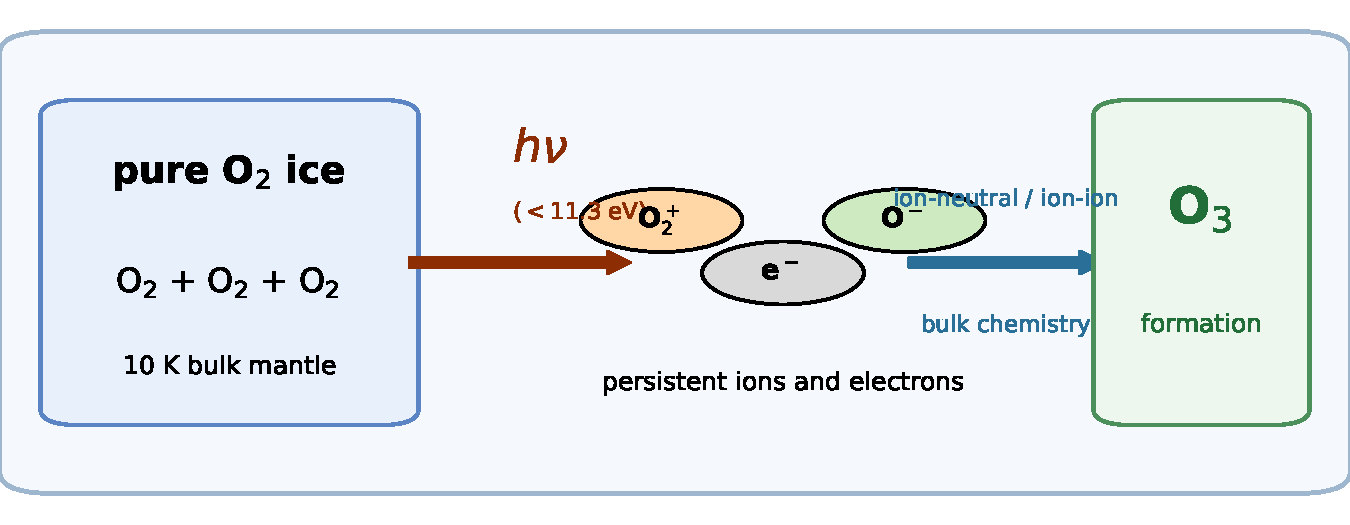
\includegraphics[width=9cm,height=3.5cm,keepaspectratio]{toc_ionice}

\noindent
UV photons ($<$11.3\,eV) ionize a pure O$_2$ ice, generating cations, anions,
and free electrons that participate in a network of bulk ion--ice reactions.
For the first time, such ionic species are explicitly tracked in an
astrochemical model, revealing the critical role of O$_3^+$ in the formation
of interstellar ozone.

\end{tocentry}

%%%%%%%%%%%%%%%%%%%%%%%%%%%%%%%%%%%%%%%%%%%%%%%%%%%%%%%%%%%%%%%%%%%%%
%% The abstract environment will automatically gobble the contents
%% if an abstract is not used by the target journal.
%%%%%%%%%%%%%%%%%%%%%%%%%%%%%%%%%%%%%%%%%%%%%%%%%%%%%%%%%%%%%%%%%%%%%
\begin{abstract}
Although energetic and non-energetic processing of interstellar dust grain surfaces and ice is thought to be one of the dominant mechanisms for the extraterrestrial synthesis of prebiotic molecules, the role that ``ion-ice'' chemistry (bulk ion-neutral and ion-ion reactions within the dust-grain ice mantle) plays is still a largely unexplored topic. In this work, we present results of our study to investigate the astrochemical importance of ions produced within dust grain ice mantles via irradiation by ionizing radiation such as cosmic rays, VUV photons, and X-rays. To this end, we present new models of the chemical evolution of a pure oxygen ice irradiated by UV photons, using a chemical network that explicitly includes bulk reactions involving secondary ions. A comparison of our calculations with previous data suggests that ion-neutral reactions (including ion-molecule and ion-ion processes) may play a critical role in understanding the chemistry of interstellar ice.
\end{abstract}

%%%%%%%%%%%%%%%%%%%%%%%%%%%%%%%%%%%%%%%%%%%%%%%%%%%%%%%%%%%%%%%%%%%%%
%% Start the main part of the manuscript here.
%%%%%%%%%%%%%%%%%%%%%%%%%%%%%%%%%%%%%%%%%%%%%%%%%%%%%%%%%%%%%%%%%%%%%
\section{Introduction}

It has now been more than half a century since the publication of the pioneering work of \citet{herbst_formation_1973}, which arguably marked the genesis of the field of astrochemical modeling. A number of key predictions from that work have since been verified. Among these was the claim that gas-phase ion-neutral reactions, beginning with those involving \ce{H3+}, were essential to the formation of polyatomic molecules in interstellar environments. These reactions are often both barrierless and exothermic, making them efficient even in dense molecular clouds, which are typically around 10 K (see the review by \citet{ceccarelli_organic_2022} and references therein for more details). In addition, especially for cases where the neutral reactant is polar, the long-range forces involved mean that such reactions can have a negative temperature dependence \citep{woon_quantum_2009} and rate coefficients significantly larger than that predicted by the Langevin equation\citep{hammes_principles_1978} of $\sim10^{-9}$ cm$^3$ s$^{-1}$. 

Just as ions are critical for the formation of polyatomic molecules in the gas phase, so too are interstellar dust grains. In interstellar environments, dust acts as a quasi-catalyst for chemical reactions. In diffuse and translucent molecular clouds, the surfaces of the bare grains act as important reaction sites, especially for the formation of \ce{H2} \citep{katz_molecular_1999,cazaux_molecular_2002,iqbal_h2_2014,acharyya_effect_2020}. So too are the ice mantles which form on dust grains in dense molecular clouds. 
Our understanding of the importance of dust-grain ice mantles in explaining the observed chemical complexity of interstellar environments has grown over the history of astrochemistry. Grain-related processes are now thought to be critical in explaining the presence of Terrestrial-like saturated or semi-saturated organic species, including ``prebiotic'' molecules which may be implicated in the origins of life on Earth and possibly elsewhere \citep{ceccarelli_organic_2022}. Nevertheless, the addition of surface and bulk ice-mantle grain chemistry, though doubtless a more accurate representation of chemistry in the real interstellar medium, remains an active area of research.

The unfortunate combination of the importance of grain-related processes in the interstellar medium (ISM), combined with a comparative lack of knowledge and data regarding relevant processes has led one astrochemical modeler to make the now well-known jest that interstellar grain chemistry represents the ``last refuge of the scoundrel\citep{charnley_molecular_1992}.''  Here, we will highlight just a few of the current areas of uncertainty that pose challenges for ice modeling, generally.  Firstly, there exist substantial uncertainties regarding the physisorption binding energies of most of the hundreds of species usually included in grain-chemical networks \citep{cuppen_modelling_2011,lamberts_influence_2017,wakelam_binding_2017}. These binding energies, which have a range of values depending on many factors, one example being the local surface morphology, are typically approximated with a single value, with some very recent exceptions\citep{grassi_novel_2020,furuya_framework_2024}.  Moreover, though it is now well established both via experiments and theory that grain and ice-mantle surface chemistry is dominated by diffusive Langmuir-Hinshelwood type reactions \citep{qasim_experimental_2020,ioppolo_non-energetic_2020,cuppen_grain_2017,watanabe_efficient_2002}, whether and how chemistry within the ice mantle occurs at low temperatures has been the subject of considerable recent work. There is a growing consensus that non-diffusive processes almost certainly play a key role \citep{theule_thermal_2013,ghesquiere_diffusion_2015,shingledecker_simulating_2019, mullikin_condensed-phase_2018,jin_formation_2020,ioppolo_non-energetic_2021}.  Finally, and most pertinent for this work, the chemical networks used for simulating interstellar grain chemistry have historically included only neutral species.

That ion-ice processes can occur efficiently under interstellar conditions was suggested in the pioneering theoretical study of \citet{woon_ion-ice_2011}, who found that cations such as \ce{HCO+} and \ce{CH3+} were able to react barrierlessly with water molecules in ice via pathways that could lead to formic acid and methanol, two astrochemically-relevant species (see also \citet{woon_quantum_2021}).  The reaction between low-energy \ce{CH3+} cations and water ice was investigated in detail by \citet{nakai_methanol_2023}, who confirmed experimentally that the reaction suggested by \citet{woon_ion-ice_2011} does indeed occur under interstellar conditions.  In that work, astrochemical models using the code of \citet{furuya_water_2015} found that the \ce{CH3+}-ice reaction was competitive at the edges of the simulated molecular cloud where the visual extinction was low, and calculated enhanced abundances of gas-phase \ce{CH3+}. 

The adsorption of gas-phase cations undoubtedly also occurs in real interstellar environments. The interaction between gas-phase cations and ice surfaces was the subject of a recent modeling study by \citet{cui_exploring_2024}, who found that such reactions could be efficient in forming complex species. However, there exist other mechanisms for driving ion-ice chemistry. 

While externally produced energetic photons are quickly extinguished in molecular clouds, galactic cosmic rays reach even the centers of most dense molecular clouds\citep{ivlev_penetration_2018}, and are an important source of continuous ice processing in the ISM \citep{strazzulla_ion_2009,dartois_cosmic_2018}.  The essential role of cosmic rays to astrochemistry has been recognized from the outset of astrochemical modeling in the first model of \citet{herbst_formation_1973}. They noted that cosmic rays drive the formation of \ce{H3+} via collisions with \ce{H2}, which also generate an internal flux of UV photons. These photons can further ionize gaseous species in molecular clouds \citep{prasad_uv_1983}.  Direct cosmic ray collisions with dust grains and their ice mantles similarly result in the formation of charged species within a roughly cylindrical region known as the ``track'' \citep{shingledecker_cosmic-ray_2020} which forms around the path of the cosmic ray through the solid.  Bombardment by internal UV photons represents yet another means of ionizing \citep{mullikin_new_2021}, albeit with a lower efficiency than with cosmic rays \citep{wu_role_2024}.  Although some fraction of the charged species produced within ices undoubtedly undergo rapid neutralization by recombination \citep{shingledecker_general_2018,woon_formation_2024}, the remainder may participate in an internal ion-ice chemistry whose importance may be comparable to that known to occur in the gas-phase. The ionization of an ice-mantle species creates, in addition to the atomic or molecular ion, a secondary electron, which can subsequently multiply the chemical effects. When such secondary electrons lose sufficient energy through collisions with bulk species, they can become ``low-energy'' electrons ($<$20 eV), which can have significant effects of their own \citep{arumainayagam_low-energy_2010,boamah_low-energy_2014,boyer_role_2016,wu_role_2024}.

In this work, we present the first computational study of secondary ion-ice chemistry driven by the UV photon ($<11.3$ eV) bombardment of a cosmic ice analogue of pure molecular oxygen, following the experimental work of \citet{gerakines_ultraviolet_1996}. \textbf{Though galactic cosmic rays are indeed the ultimate drivers of ion chemistry (both gas and solid phase) in dense molecular clouds, they generate an internal flux of VUV photons which trigger a broadly similar set of reactions as the cosmic rays themselves. It is these VUV photons which we simulate in this work, following the laboratory conditions of \citet{gerakines_ultraviolet_1996}.} \textbf{The key distinction between the present work and all our previous implementations of this modeling approach \citep{shingledecker_general_2018,mullikin_new_2021} is our relaxation of the requirement that ionization always proceed via pathway R2---that is, ionization followed immediately by charge recombination, such that in previous studies, ionic species were never present in the simulated ice. Here, for the first time, we allow ionization to proceed via pathway R1, yielding long-lived ionic species that participate in a network of ion--neutral, ion--ion, and dissociative recombination reactions within the bulk ice. Thus, the three primary innovations of this work are: (i) the first astrochemical kinetic model to include cations, anions, and free electrons as persistent species within the bulk ice mantle, allowing them to undergo non-diffusive ion–neutral, ion–ion, and dissociative recombination reactions in the solid phase.  (ii) two new kinetic parameters, $\nu_\mathrm{i-n}$ and $\nu_\mathrm{i-i}$, extending the non-diffusive rate formalism of \citet{shingledecker_simulating_2019} to charged species; and (iii) the first computational study of secondary ion chemistry in a UV-irradiated cosmic ice analogue. We note, regarding point (i), that this is distinct from recent models treating Eley–Rideal reactions of gas-phase ions with ice surfaces \citep{cui_exploring_2024}, which do not include internally generated bulk ionic species.} Our paper is laid out as follows: in \S\ref{sec:theory} we describe our theoretical and computational approach, in \S\ref{sec:results} we present the results of our trials and describe their astrochemical significance, and finally, we summarize our findings in \S\ref{sec:conclusions}. 

\section{Theory} \label{sec:theory}

\subsection{Formation of Ions Within Cosmic Ice}\label{sec:ionformation}

Here, we are focused on the chemical contribution of ions produced within cosmic ice. In dense molecular clouds, as noted in the introduction, there exist two main mechanisms which could drive the ionization of dust-grain ice mantle species; namely, galactic cosmic rays\citep{silsbee_magnetic_2018,ivlev_penetration_2018} and the UV photons they generate through the excitation of \ce{H2}\citep{prasad_uv_1983}. The basis of the theoretical approach used in our models is that of \citet{shingledecker_general_2018}, which begins with the assumption of a set of four possible outcomes when some ice constituent, \ce{A}, encounters some particle of ionizing radiation:

\begin{align}
    aA &\leadsto{} aA^+ + e^- 
\tag{R1}
\label{r1}\\
aA &\leadsto{} aA^+ + e^- \rightarrow{} aA^* \rightarrow{} bB^* + cC^* 
\tag{R2}
\label{r2}\\
aA &\leadsto{} aA^* \rightarrow{} bB + cC 
\tag{R3}
\label{r3}\\
aA &\leadsto{} aA^*
\tag{R4}
\label{r4}
\end{align}


\noindent
where the lower case letters represent the relevant stoichiometric coefficients. Processes \eqref{r1} and \eqref{r2} correspond to the ionization of \ce{A}, while \eqref{r3} and \eqref{r4} represent the effects of excitation to a higher vibrational or electronic state. \citet{shingledecker_general_2018} furthermore derive expressions for the rate coefficients \eqref{r1} - \eqref{r4}, albeit for cases where the \ce{A} encounters a particle such as an energetic proton. This formalism was later expanded by Shingledecker et al. \citep{mullikin_new_2021} to treat irradiation by photons. 

In large part because grain-chemical networks have only included neutral species, previous modeling works using one of the above approaches have made the assumption that in every case, the ionization of \ce{A} proceeds via \eqref{r2} rather than \eqref{r1}, i.e., that ionization is followed by rapid charge recombination to yield some excited suprathermal products. In contrast, here we assume as a first-order approximation that the two ionization processes, \eqref{r1} and \eqref{r2}, occur with equal probability.

Briefly, to obtain rate coefficients ($k_\mathrm{photo}$) for \eqref{r1} - \eqref{r4}, we begin with the standard formula for photo-processes:

\begin{equation}
    k_\mathrm{photo} = \int \sigma(\lambda)I(\lambda) d\lambda
    \label{eq:kphotostandard}
\end{equation}

\noindent  
where the resulting value is a function of the wavelength-dependent absorption cross-sections ($\sigma(\lambda)$) and intensities ($I(\lambda)$) integrated over all wavelengths \citep{van_dishoeck_photodissociation_1988}. To obtain the ultimately-utilized expression for the rate coefficients, we express Eq. \eqref{eq:kphotostandard} as

\begin{equation}
    k_\mathrm{photo} = \frac{\int \sigma(\lambda)I(\lambda)d\lambda}{\int I(\lambda)d\lambda} \int I(\lambda)d\lambda = \Bar{\sigma}\Phi
    \label{eq:kmullikin}
\end{equation}

\noindent
such that the rate coefficient can be written as the product of an average cross section for a given species and the photon flux integrated over all wavelengths. 

As given in \citet{mullikin_new_2021}, the individual $k_\mathrm{photo}$ values for \eqref{r1} - \eqref{r4} are then multiplied by some branching fractions, $f_\mathrm{br}$. For a given species, we divide the branching fractions such that all ionization processes for that species add to unity (Type R1 and R2 in Table 1), and all excitation processes (R3 and R4) for a given species likewise add to unity.

Mullikin et al. also introduces the factor $\delta$, which accounts for any discrepancy due to unavailable data, such as the difference between the actual solid phase cross-sections compared with the gas-phase values used here. Thus, the rate coefficients for photo-driven processes in our model are given by

\begin{equation}
    k_\mathrm{photo} = f_\mathrm{br}\Bar{\sigma}\Phi\delta.
\end{equation}

\noindent
Shown in Table \ref{tbl:network_photo} are the cross sections and branching fractions for the various processes used here, taken from \citet{mullikin_new_2021}. Each separate process in that table is given a label prefixed with ``P'' while the generic type of process using the four pathways given above and described in \citet{shingledecker_new_2017} are denoted R1 to R4. For ionization processes, the total branching fraction is split between pathway types R1 and R2, where applicable. Likewise for excitation, branching fractions are split between R3 and R4. Though gas-phase molecular oxygen has an ionization energy of $\sim$ 12 eV, slightly higher than the UV photon energies used by \citet{gerakines_ultraviolet_1996}, these values are typically lowered by a few eV in solids, leading to a non-zero cross section for processes P2 and P3. \textbf{We note that processes P7 and P10 share the same net stoichiometry (\ce{O} $\leadsto$ \ce{O^*}) but represent fundamentally distinct physical mechanisms with different rate expressions. P7 is an R2-type process (ionization of \ce{O} followed immediately by charge recombination), whose rate is proportional to the ionization cross section of \ce{O}; since the ionization potential of atomic oxygen (13.6~eV) exceeds the maximum photon energy employed here, this cross section is effectively zero. P10 is an R3-type process (direct electronic excitation of \ce{O} without ionization), which in principle carries a non-zero excitation cross section. The identical net reaction therefore reflects two distinct physical channels, not a duplication.}

\begin{table*}[tb!]
  \caption{Photoprocesses included in our model}
  \label{tbl:network_photo}
 \begin{tabular}{l l c c l  c  c }
 \hline
 Number & Type &  & Process &  & $f_\mathrm{br}$ & $ \Bar{\sigma}$ (cm$^{2}$) \\ 
 \hline
 %R1 Ionization Processes
 \pcount{plabel1} &   R1  & \ce{O}  & $\leadsto$ & \ce{O+} + \ce{e-}    & 0.50 & 0.00                 \\
 \pcount{plabel2} &   R1  & \ce{O2} & $\leadsto$ & \ce{O+} + \ce{O-}    & 0.25 & $3.86\times10^{-20}$ \\
 \pcount{plabel3} &   R1  & \ce{O2} & $\leadsto$ & \ce{O2+} + \ce{e-}   & 0.25 & $3.86\times10^{-20}$ \\
 \pcount{plabel4} &   R1  & \ce{O3} & $\leadsto$ & \ce{O+} + \ce{O2-}   & 0.167 & 0.00                 \\
 \pcount{plabel5} &   R1 & \ce{O3} & $\leadsto$  & \ce{O2+} + \ce{O-}   & 0.167 & 0.00                 \\
 \pcount{plabel6} &   R1 & \ce{O3} & $\leadsto$  & \ce{O3+} + \ce{e-}   & 0.167 & 0.00                 \\
 %R2 Ionization Processes
 \pcount{plabel7} &   R2  & \ce{O} & $\leadsto$  & \ce{O^*}             & 0.50 & 0.00                 \\
 \pcount{plabel8} &   R2  & \ce{O2} & $\leadsto$ & \ce{O^*} + \ce{O^*}  & 0.50 & $3.86\times10^{-20}$ \\
 \pcount{plabel9} &   R2  & \ce{O3} & $\leadsto$ & \ce{O2^*} + \ce{O^*} & 0.50 & 0.00                 \\
 %R3 Excitation Processes
 \pcount{plabel10} &   R3 & \ce{O} & $\leadsto$   & \ce{O^*}             & 1.00 & 0.00                 \\
 \pcount{plabel11} &   R3 & \ce{O2} & $\leadsto$  & \ce{O2^*}            & 0.50 & $2.13\times10^{-18}$ \\
 \pcount{plabel12} &   R3 & \ce{O3} & $\leadsto$  & \ce{O3^*}            & 0.50 & $5.60\times10^{-18}$ \\
 %R4 Excitation Processes
 \pcount{plabel13} &   R4 & \ce{O2} & $\leadsto$  & \ce{O} + \ce{O}      & 0.50 & $2.13\times10^{-18}$ \\
 \pcount{plabel14} &   R4 & \ce{O3} & $\leadsto$  & \ce{O2} + \ce{O}     & 0.50 & $5.60\times10^{-18}$ \\
 \hline
 \end{tabular}
\end{table*}


\subsection{The Chemistry of Solid-Phase Ions}\label{sec:ionchem}

Thus formed within the ice as described in \S\ref{sec:ionformation}, the ions in our simulations are allowed to react chemically. Whether, or by which mechanism, reactions occur in low-temperature cosmic ice is still a matter of ongoing investigation. Here we assume, as in \citet{shingledecker_simulating_2019}, that rapid reactions can and do occur between neighbors even at temperatures as low as 5 K, in other words, non-diffusively. This approach was motivated by a now large body of experimental studies showing persuasively that even complex organic molecules (COMs) can be formed via fast solid-phase non-diffusive reactions \citep{abplanalp_study_2016,doddipatla_low-temperature_2021,bergantini_combined_2018,jin_formation_2020,mullikin_condensed-phase_2018,ghesquiere_reactivity_2018} and, when incorporated into simulations of astrophysical environments, yield predicted abundances of ice-mantle species that have proven to be in general agreement with recent JWST observations \citep{shingledecker_efficient_2020,mcclure_ice_2023,yang_corinos_2022}. 

As described in \citet{shingledecker_simulating_2019}, the fast non-diffusive bulk rate coefficient for some reaction \ce{A + B} is given by

\begin{equation}
    k_\mathrm{fast} = f_\mathrm{br}\left[\frac{\nu_0^\mathrm{A} + \nu_0^\mathrm{B}}{n_\mathrm{bulk}} \right] \mathrm{exp}\left( - \frac{E_\mathrm{act}^{AB}}{T_\mathrm{ice}}\right)
    \label{kfast}
\end{equation}

\noindent
where, $\nu_0^\mathrm{A}$ and $\nu_0^\mathrm{B}$ are the vibrational frequencies of A and B, $n_\mathrm{bulk}$ is the number of species in the ice mantle, exclusive of the surface layers, $E_\mathrm{act}$ is the activation energy in units of Kelvin, if present, and $T_\mathrm{ice}$ is the ice temperature. If one of the vibrational frequencies is much larger than the other, for example where $\nu_0^\mathrm{A} \gg \nu_0^\mathrm{B}$, then Eq. \eqref{kfast} can be simplified to

\begin{equation}
    k_\mathrm{fast} \approx f_\mathrm{br}\left[\frac{\nu_\mathrm{n-n}}{n_\mathrm{bulk}} \right] \mathrm{exp}\left( - \frac{E_\mathrm{act}^{AB}}{T_\mathrm{ice}}\right)
    \label{kfast2}
\end{equation}

\noindent
where $\nu_\mathrm{n-n} = \nu_0^\mathrm{A}$. Hereafter, we will refer to $\nu_\mathrm{n-n}$ as the neutral-neutral trial frequency.

As originally described in \citet{shingledecker_simulating_2019}, the species undergoing fast solid-phase reactions were all neutrals. For the purposes of this work, we have modified Eq. \eqref{kfast} slightly to also treat the solid-phase reaction of ions. First, for reactions between ions and neutrals of the forms \ce{A+ + B} and \ce{A + B-}, we replace $\nu_\mathrm{n-n}$ with another frequency $\nu_\mathrm{i-n}$, the ion-neutral trial frequency. Finally, for reactions between two charged species of the form \ce{A+ + B-}, we invoke a third frequency, $\nu_\mathrm{i-i}$, the ion-ion trial frequency. Here, the anions do not form directly from any of the processes in Table \ref{tbl:network_photo}, but rather, result from, e.g., electron attachment reactions. The three frequencies in Eq. \eqref{kfast2} represent the different long-range forces experienced between the reactants and account for the potentially higher overall reaction rate between a cation and an anion relative to a reaction involving two neutral species, even in an environment where diffusion is severely inhibited. As we describe in \S\ref{sec:results}, these three frequencies were varied in our models to ascertain their influence on the resulting predicted abundances. As noted by \citet{theule_thermal_2013}, the order of magnitude of the pre-exponential frequencies can vary widely, depending on the underlying mechanism and phase where reactions are occurring, e.g. gas or liquid. The same work further notes an enormous possible range of values for first-order processes between $10^{13}$ s$^{-1}$ in the gas phase to as low as $\sim10^{-3}$ s$^{-1}$ in other cases, with those in condensed media being lower. The underlying causes for such variation are not, as far as we know, currently understood but could be related to effects such as the entropy of activation. \cb{A physically plausible interpretation is that such variation reflects the strong configurational constraints imposed by the condensed-phase environment. In transition-state-theory language, this could manifest as an effective entropy-of-activation effect, though we do not regard that explanation as unique here \citep{theule_thermal_2013}.}

\subsection{Model \& Chemical Network}

\subsubsection{Reaction Network}

\begin{table*}[htbp]
\centering
\footnotesize
\caption{The base chemical network used to model solid-phase \ce{O2} photo-processing and subsequent chemistry, taken from \citet{mullikin_new_2021} and \citet{shingledecker_simulating_2019}.}
\label{tab:onetwork}
\begin{tabular}{lll}
\toprule
\multicolumn{3}{c}{Non-Photon-Induced Reactions} \\
\midrule
$\ce{O3^*} + \ce{O3} \rightarrow \ce{O2} + \ce{O2} + \ce{O2}$ &
$\ce{O2^*} + \ce{O} \rightarrow \ce{O3^*}$ &
$\ce{O^*} + \ce{O3^*} \rightarrow \ce{O2} + \ce{O2}$ \\

$\ce{O} + \ce{O} \rightarrow \ce{O2^*}$ &
$\ce{O2^*} + \ce{O} \rightarrow \ce{O2} + \ce{O}$ &
$\ce{O2^*} + \ce{O2^*} \rightarrow \ce{O2} + \ce{O2}$ \\

$\ce{O^*} + \ce{O} \rightarrow \ce{O} + \ce{O}$ &
$\ce{O2^*} + \ce{O2} \rightarrow \ce{O2} + \ce{O2}$ &
$\ce{O2^*} + \ce{O3^*} \rightarrow \ce{O2} + \ce{O2} + \ce{O}$ \\

$\ce{O^*} + \ce{O} \rightarrow \ce{O2^*}$ &
$\ce{O2^*} + \ce{O3} \rightarrow \ce{O2} + \ce{O2} + \ce{O}$ &
$\ce{O3^*} + \ce{O3^*} \rightarrow \ce{O2} + \ce{O2} + \ce{O2}$ \\

$\ce{O^*} + \ce{O2} \rightarrow \ce{O3^*}$ &
$\ce{O^*} + \ce{O^*} \rightarrow \ce{O} + \ce{O}$ &
$\ce{O} + \ce{O3^*} \rightarrow \ce{O2} + \ce{O2}$ \\

$\ce{O^*} + \ce{O2} \rightarrow \ce{O} + \ce{O2}$ &
$\ce{O^*} + \ce{O2^*} \rightarrow \ce{O3^*}$ &
$\ce{O2} + \ce{O3^*} \rightarrow \ce{O2} + \ce{O2} + \ce{O}$ \\

$\ce{O} + \ce{O3} \rightarrow \ce{O2} + \ce{O2}$ &
$\ce{O^*} + \ce{O2^*} \rightarrow \ce{O} + \ce{O2}$ &
$\ce{O} + \ce{O2} \rightarrow \ce{O3^*}$ \\

$\ce{O^*} + \ce{O3} \rightarrow \ce{O2} + \ce{O2}$ & & \\
\bottomrule
\end{tabular}
\end{table*}

The reaction network in this work was limited to oxygen species only, since it is arguably the simplest radiation-chemical system, and for which there exist relevant experimental data in the work of \citet{gerakines_ultraviolet_1996}. \textbf{We note that a number of additional experimental studies of photolysis and radiolysis of pure oxygen ice are relevant to the broader context of this network. In particular, \citet{zhen_uv-induced_2014} report UV-photodesorption and photochemistry cross sections for O$_2$ ice, and \citet{sivaraman_temperature-dependent_2007} examine the temperature-dependent formation of ozone under 5~keV electron irradiation; the ozone yields reported in both works are qualitatively consistent with the photochemical pathways included in our model, and both works are in broad agreement with our findings, described below, regarding the dominant chemical pathways to ozone formation. } The starting point for our network was the oxygen network in \citet{mullikin_new_2021}, shown in Table \ref{tab:onetwork}, which in turn was based on previous work by \citet{shingledecker_simulating_2019} and \citet{shingledecker_new_2017}. Our base network \citep{mullikin_new_2021}, which included only reactions between neutral species, was expanded with the reactions shown in Table \ref{tbl:network_rxn} to include charge recombination reactions of the form

\begin{equation}
    \ce{A+ + B- -> C + D}
\end{equation}

\noindent
using the reaction networks in \citet{pastina_effect_2001}, \citet{anicich_index_2003}, and the NIST Chemical WebBook\footnote{https://webbook.nist.gov/chemistry/}. We further added two more classes of reactions involving two species with unlike charges; namely, ion-ion recombination of the form

\begin{equation}
    \ce{A+ + B- -> C^*} + \ce{D^*}
\end{equation}

\noindent
and dissociative recombination between cations and electrons of the form

\begin{equation}
    \ce{A+ + e- -> C^*} + \ce{D^*}
\end{equation}

\noindent
In both of the two cases above, we assume that the products are created in an excited suprathermal state, given the high exothermicity of the process. All new reactions involving ions were assumed to proceed barrierlessly. \cb{These ion-induced reactions enter the standard rate-equation formalism as additional formation and destruction terms, with rate coefficients given by Eq.~\eqref{kfast2} using the ionic trial frequencies $\nu_\mathrm{i-n}$ or $\nu_\mathrm{i-i}$ as appropriate, and with $E_\mathrm{act} = 0$ for all charged-species reactions. UV photolysis is included explicitly via the photoprocess rate coefficients in Table~\ref{tbl:network_photo}, which compete with all chemical reactions at each timestep. Thermal diffusion is deliberately excluded: our non-diffusive framework (Section~\ref{sec:ionchem}) is motivated by experimental evidence that bulk ice reactions can occur even at temperatures where thermal diffusion is negligible. Grain-surface reactions are not included, as the model describes bulk ice chemistry only. We also note that the present model assumes spatially uniform (homogeneous) chemical processing throughout the ice mantle, which is a fundamental limitation of standard rate-equation astrochemical models, though the region over which abundances are averaged can be subdivided as in the multilayer model of \citet{taquet_multilayer_2012} and \citet{vasyunin_formation_2017}. In the context of UV-photon irradiation, where energy is deposited relatively uniformly over the penetration depth of thin ice films, this assumption is better justified than it would be for MeV heavy-ion bombardment, where spatial inhomogeneity along ion tracks can be significant. Sputtering, compaction, and structural modifications of the ice are not modeled in this work, though future extensions of this technique could begin to account for them systematically.}


\begin{table*}[p!]
    \footnotesize
    \caption {New reactions involving charged species added for this work.} 
    \label{tbl:network_rxn}
 \begin{tabular}{l r c l c  }
 \hline
 Number & & Reaction &  & Branching Fraction  \\ 
 \hline
 \ncount{nlabel3} & \ce{O} + \ce{e-} & $\rightarrow$ & \ce{O-} &  1.00      \\
 %%%
 \ncount{nlabel4} & \ce{O} + \ce{O-} & $\rightarrow$ & \ce{O2-} & 1.00       \\
 %%%
 \ncount{nlabel5} & \ce{O} + \ce{O2-} & $\rightarrow$ & \ce{O3-} & 1.00      \\
 %%%
 \ncount{nlabel6} & \ce{O+} + \ce{e-} & $\rightarrow$ & \ce{O^*} & 1.00     \\
 %%%
 \ncount{nlabel7} & \ce{O+} + \ce{O-} & $\rightarrow$ & \ce{O2^*} & 0.50      \\
 %%%
 \ncount{nlabel8} & \ce{O+} + \ce{O-} & $\rightarrow$ & \ce{O^*} + \ce{O^*} & 0.50     \\
 %%%
 \ncount{nlabel9} & \ce{O+} + \ce{O2} & $\rightarrow$ & \ce{O2+} + \ce{O} & 1.00      \\
 %%%
 \ncount{nlabel10} & \ce{O+} + \ce{O2-} & $\rightarrow$ & \ce{O3^*} &  0.50       \\
 %%%
 \ncount{nlabel11} & \ce{O+} + \ce{O2-} & $\rightarrow$ & \ce{O^*} + \ce{O2^*} & 0.50       \\
 %%%
 \ncount{nlabel12} & \ce{O+} + \ce{O3-} & $\rightarrow$ & \ce{O^*} + \ce{O3^*} & 0.50       \\
 %%%
 \ncount{nlabel13} & \ce{O+} + \ce{O3-} & $\rightarrow$ & \ce{O2^*} + \ce{O2^*} & 0.50        \\
 %%%
 \ncount{nlabel14} & \ce{O2} + \ce{e-} & $\rightarrow$ & \ce{O2-} &  1.00  \\
 %%%
 \ncount{nlabel15} & \ce{O2} + \ce{O-} & $\rightarrow$ & \ce{O3-} & 1.00   \\
 %%%
 \ncount{nlabel16} & \ce{O2+} + \ce{e-} & $\rightarrow$ & \ce{O2^*} &  0.50   \\
 %%%
 \ncount{nlabel17} & \ce{O2+} + \ce{e-} & $\rightarrow$ & \ce{O^*} + \ce{O^*} & 0.50    \\
 %%%
 \ncount{nlabel18} & \ce{O2+} + \ce{O-} & $\rightarrow$ & \ce{O3^*} & 0.50    \\
 %%%
 \ncount{nlabel19} & \ce{O2+} + \ce{O-} & $\rightarrow$ & \ce{O^*} + \ce{O2^*} & 0.50     \\
 %%%
 \ncount{nlabel20} & \ce{O2+} + \ce{O2} & $\rightarrow$ & \ce{O3+} + \ce{O} & 1.00  \\
 %%%
 \ncount{nlabel21} & \ce{O2+} + \ce{O2-} & $\rightarrow$ & \ce{O^*} + \ce{O3^*} & 0.50    \\
 %%%
 \ncount{nlabel22} & \ce{O2+} + \ce{O2-} & $\rightarrow$ & \ce{O2^*} + \ce{O2^*} & 0.50    \\
 %%%
 \ncount{nlabel23} & \ce{O2+} + \ce{O3-} & $\rightarrow$ & \ce{O2^*} + \ce{O3^*} &  0.33    \\
 %%%
 \ncount{nlabel24} & \ce{O2+} + \ce{O3-} & $\rightarrow$ & \ce{O2^*} + \ce{O2^*} + \ce{O^*} & 0.33   \\
 %%%
 \ncount{nlabel25} & \ce{O2+} + \ce{O3-} & $\rightarrow$ & \ce{O3^*} + \ce{O^*} + \ce{O^*} & 0.33   \\
 %%%
 \ncount{nlabel26} & \ce{O3} + \ce{e-} & $\rightarrow$ & \ce{O3-} & 1.00  \\
 %%%
 \ncount{nlabel27} & \ce{O3} + \ce{O-} & $\rightarrow$ & \ce{O2-} + \ce{O2} & 1.00   \\
 %%%
 \ncount{nlabel28} & \ce{O3} + \ce{O2-} & $\rightarrow$ & \ce{O3-} + \ce{O2} & 1.00  \\
 %%%
 \ncount{nlabel29} & \ce{O3} + \ce{O3+} & $\rightarrow$ & \ce{O2} + \ce{O2} + \ce{O2+} & 1.00    \\
 %%%
 \ncount{nlabel30} & \ce{O3-} + \ce{O-} & $\rightarrow$ & \ce{O2-} + \ce{O2-} & 1.00   \\
 %%%
 \ncount{nlabel31} & \ce{O3+} + \ce{e-} & $\rightarrow$ & \ce{O3^*} & 0.50   \\
 %%%
 \ncount{nlabel32} & \ce{O3+} + \ce{e-} & $\rightarrow$ & \ce{O2^*} + \ce{O^*} & 0.50  \\
 %%%
 \ncount{nlabel33} & \ce{O3+} + \ce{O-} & $\rightarrow$ & \ce{O^*} + \ce{O3^*} &  0.50   \\
 %%%
 \ncount{nlabel34} & \ce{O3+} + \ce{O-} & $\rightarrow$ & \ce{O2^*} + \ce{O2^*} & 0.50  \\
 %%%
 \ncount{nlabel35} & \ce{O3+} + \ce{O2} & $\rightarrow$ & \ce{O2+} + \ce{O3} & 0.415    \\
 %%%
 \ncount{nlabel36} & \ce{O3+} + \ce{O2} & $\rightarrow$ & \ce{O3+} + \ce{O2} & 0.085   \\
 %%%
 \ncount{nlabel37} & \ce{O3+} + \ce{O2} & $\rightarrow$ & \ce{O2} + \ce{O2} + \ce{O+} & 0.50  \\
 %%%
 \ncount{nlabel38} & \ce{O3+} + \ce{O2-} & $\rightarrow$ & \ce{O2^*} + \ce{O3^*} & 0.33   \\
 %%%
 \ncount{nlabel39} & \ce{O3+} + \ce{O2-} & $\rightarrow$ & \ce{O2^*} + \ce{O2^*} + \ce{O^*} & 0.33  \\
 %%%
 \ncount{nlabel40} & \ce{O3+} + \ce{O2-} & $\rightarrow$ & \ce{O3^*} + \ce{O^*} + \ce{O^*} & 0.33  \\
 %%%
 \ncount{nlabel41} & \ce{O3+} + \ce{O3-} & $\rightarrow$ & \ce{O3^*} + \ce{O3^*} & 0.33  \\
 %%%
 \ncount{nlabel42} & \ce{O3+} + \ce{O3-} & $\rightarrow$ & \ce{O3^*} + \ce{O2^*} + \ce{O^*} & 0.33  \\
 %%%
 \ncount{nlabel43} & \ce{O3+} + \ce{O3-} & $\rightarrow$ & \ce{O2^*} + \ce{O2^*} + \ce{O2^*} & 0.33  \\
 %%%
 \hline
 \end{tabular}
\end{table*}

\subsection{Model Parameters}

In order to examine the role of condensed-phase ion-molecule reactions under well-constrained conditions, we have simulated previous laboratory experiments directly, rather than an interstellar region. Specifically, we have sought to reproduce the experiments reported in \citet{gerakines_ultraviolet_1996}, which studied the effects of irradiating a pure molecular oxygen ice deposited on a \ce{MgF2} substrate at a temperature of 10 K with UV photons ($<11.3$ eV) from a microwave-discharge hydrogen lamp (MHDL) \textbf{with a photon flux of $2.2\times10^{14}$ photons cm$^{-2}$ s$^{-1}$ as reported in \citet{gerakines_ultraviolet_1996}. We note that though this is a direct simulation of an experiment, this method could be easily extended to real interstellar sources via, e.g. adjusting the flux to an appropriate ISM value. }

Here, a suite of simulations were carried out to simulate this ice irradiation using a variety of kinetic parameters, with the goal of understanding the dependence of the underlying chemistry on these values. A full list of the models run, and the values of the varied parameters, is given in Table \ref{tbl:parameters}.

\begin{table*}[p!]
  \centering
    \footnotesize
  \caption{Model sets described here, and their associated parameters.}
  \label{tbl:parameters}
  \begin{tabular}{cccc}
    \hline
     Model & $\nu_{n-n}$  & $\nu_{i-n}$ & $\nu_{i-i}$ \\
     & (s$^{-1}$)   &   (s$^{-1}$)&   (s$^{-1}$)\\                
    \hline
    1 & $5.00\times10^{8}$  & $3.0\times10^{7}$ & $6.93\times10^{11}$ \\
2  & \(1.00 \times 10^{13}\) & \(1.00 \times 10^{13}\) & \(1.00 \times 10^{13}\) \\
3  & \(1.00 \times 10^{13}\) & \(1.00 \times 10^{13}\) & \(1.00 \times 10^{10}\) \\
4  & \(1.00 \times 10^{13}\) & \(1.00 \times 10^{13}\) & \(1.00 \times 10^{8}\) \\
5  & \(1.00 \times 10^{13}\) & \(1.00 \times 10^{10}\) & \(1.00 \times 10^{13}\) \\
6  & \(1.00 \times 10^{13}\) & \(1.00 \times 10^{10}\) & \(1.00 \times 10^{10}\) \\
7  & \(1.00 \times 10^{13}\) & \(1.00 \times 10^{10}\) & \(1.00 \times 10^{8}\) \\
8  & \(1.00 \times 10^{13}\) & \(1.00 \times 10^{8}\) & \(1.00 \times 10^{13}\) \\
9  & \(1.00 \times 10^{13}\) & \(1.00 \times 10^{8}\) & \(1.00 \times 10^{10}\) \\
10 & \(1.00 \times 10^{13}\) & \(1.00 \times 10^{8}\) & \(1.00 \times 10^{8}\) \\
11 & \(1.00 \times 10^{10}\) & \(1.00 \times 10^{13}\) & \(1.00 \times 10^{13}\) \\
12 & \(1.00 \times 10^{10}\) & \(1.00 \times 10^{13}\) & \(1.00 \times 10^{10}\) \\
13 & \(1.00 \times 10^{10}\) & \(1.00 \times 10^{13}\) & \(1.00 \times 10^{8}\) \\
14 & \(1.00 \times 10^{10}\) & \(1.00 \times 10^{10}\) & \(1.00 \times 10^{13}\) \\
15 & \(1.00 \times 10^{10}\) & \(1.00 \times 10^{10}\) & \(1.00 \times 10^{10}\) \\
16 & \(1.00 \times 10^{10}\) & \(1.00 \times 10^{10}\) & \(1.00 \times 10^{8}\) \\
17 & \(1.00 \times 10^{10}\) & \(1.00 \times 10^{8}\) & \(1.00 \times 10^{13}\) \\
18 & \(1.00 \times 10^{10}\) & \(1.00 \times 10^{8}\) & \(1.00 \times 10^{10}\) \\
19 & \(1.00 \times 10^{10}\) & \(1.00 \times 10^{8}\) & \(1.00 \times 10^{8}\) \\
20 & \(1.00 \times 10^{8}\) & \(1.00 \times 10^{13}\) & \(1.00 \times 10^{13}\) \\
21 & \(1.00 \times 10^{8}\) & \(1.00 \times 10^{13}\) & \(1.00 \times 10^{10}\) \\
22 & \(1.00 \times 10^{8}\) & \(1.00 \times 10^{13}\) & \(1.00 \times 10^{8}\) \\
23 & \(1.00 \times 10^{8}\) & \(1.00 \times 10^{10}\) & \(1.00 \times 10^{13}\) \\
24 & \(1.00 \times 10^{8}\) & \(1.00 \times 10^{10}\) & \(1.00 \times 10^{10}\) \\
25 & \(1.00 \times 10^{8}\) & \(1.00 \times 10^{10}\) & \(1.00 \times 10^{8}\) \\
26 & \(1.00 \times 10^{8}\) & \(1.00 \times 10^{8}\) & \(1.00 \times 10^{13}\) \\
27 & \(1.00 \times 10^{8}\) & \(1.00 \times 10^{8}\) & \(1.00 \times 10^{10}\) \\
28 & \(1.00 \times 10^{8}\) & \(1.00 \times 10^{8}\) & \(1.00 \times 10^{8}\) \\
    \hline
  \end{tabular}
\end{table*}

For Model 1, we used a method for achieving optimal agreement between calculated and experimental data based on the approach used in \citet{mullikin_new_2021}. The three aforementioned trial frequencies, $\nu_{n-n}$, $\nu_{i-n}$, and $\nu_{i-i}$, as well as the $\delta$ factors for select reactions described below were allowed to vary. The overall agreement between a given model and the experimental data was characterized with the value, $\chi$, given by

\begin{equation}
    \chi = \sqrt{\frac{\sum_{i=1}^{n} (m_i - e_i)^2}{n}}
\end{equation}

\noindent
where $e_i$ and $m_i$ are the $i^{\textrm{th}}$ experimental and model data points out of a total of $n$.

Regarding the variation of $\delta$ values, the results of a sensitivity analysis carried out by us found that calculated \ce{O3} abundances were most sensitive to processes \ref{plabel2}, \ref{plabel3}, and \ref{plabel14}. Thus, for our Model 1 results, only these were allowed to vary up or down by two orders of magnitude for the sake of computational efficiency, with the others fixed at unity. 

\section{Results and discussion} \label{sec:results}

\subsection{Best-Fit Model}

In Table \ref{tbl:best_params}, we show values for the $\delta$ parameters for each photo process that yielded the best fit to experimental data. Shown in Fig. \ref{fig:gerakines_comp} are the calculated abundances for \ce{O3} vs. fluence for Model 1. Here, the fluence is defined as the product of the flux and the time. In Model 1, which resulted in \cb{$\chi = 0.484$}, the value of $\nu_\mathrm{i-i}$ is set to a value of $\sim7\times10^{11}$ s$^{-1}$, several orders of magnitude higher than the other frequency values of $\nu_\mathrm{n-n}=5\times10^{8}$ s$^{-1}$ and $\nu_\mathrm{i-n}=3\times10^7$ s$^{-1}$. This comparatively high value of $\nu_\mathrm{i-i}$, coupled with a low value for $\nu_\mathrm{i-n}$, tends toward the limiting case where ions produced in the bulk recombine very quickly, corresponding to the assumption made in our prior work where solid-phase ions were not present in the bulk \citep{shingledecker_general_2018,shingledecker_efficient_2020,mullikin_new_2021}. Previously, we assumed that ionization proceeded solely via process \eqref{r2}. The associated $\delta$ values for this model are given in Table \ref{tbl:best_params}. \cb{A comparison between the abundances of Model 1 here and the results described in \citet{mullikin_new_2021} shows broadly good agreement, as expected, though the exact parameters obtained differ somewhat due to the greatly expanded network. We note that \citet{gerakines_ultraviolet_1996} reported a peak \ce{O3}/\ce{O2} ratio of $\sim$36\%, whereas the maximum ratio reached in Model~1 is $\sim$23.5\%. This discrepancy arises because Model~1 was optimized to minimize the root-mean-square deviation $\chi$ across all data points over the full fluence range, rather than to reproduce the peak ratio at a single fluence value. The best-fit model is therefore driven by the overall temporal profile of the \ce{O3} abundance, and the lower peak value reflects this global optimization rather than a systematic failure of the model. We note as well that, in \citet{gerakines_ultraviolet_1996}, the percent conversion of \ce{O2} to \ce{O3} is stated to be 36\%, which we interpret as a percentage of the total initial oxygen atoms as in our previous study\citep{mullikin_new_2021}.}


\subsection{Other Models}

As shown in Table \ref{tbl:parameters}, in addition to Model 1, our best-fit model, we also ran a number of other simulations to investigate the effects of key parameters on the resulting agreement with experimental data. The resulting ozone abundances are shown in Fig. \ref{fig:othermodels}. In Models 2 - 28, all $\delta$ values were set to unity, while $\nu_{n-n}$, $\nu_{i-n}$, and $\nu_{i-i}$ were tested using all possible combinations of three different frequency values: low (\cb{$1.00\times 10^{8}$} s$^{-1}$), medium (\cb{$1.00\times 10^{10}$} s$^{-1}$), and high (\cb{$1.00\times 10^{13}$} s$^{-1}$). These models highlight the importance of the $\delta$ values in obtaining a good fit to the experimental data, and all of these  test simulations resulted in high fit values of $\chi>12$. In general, we found that models with higher relative values for $\nu_\mathrm{i-n}$ gave the worst agreement, in line with the findings of our best-fit model. In the following sections, the chemistry of neutrals and ions is analyzed. We focus on the results of the best-fit Model 1.








\begin{figure}[htb]
    \centering
    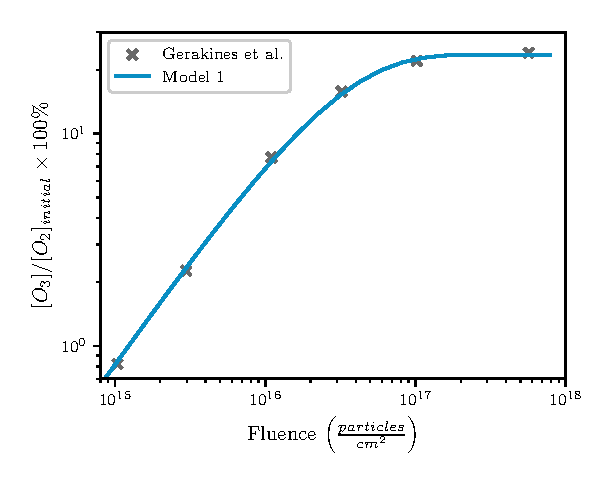
\includegraphics[width=\columnwidth]{f1.eps}
    \caption{Model 1 calculated abundances of \ce{O3} in best fit model compared with experimental data.}
    \label{fig:gerakines_comp}
\end{figure}%

\begin{figure*}[htb]
    \centering
    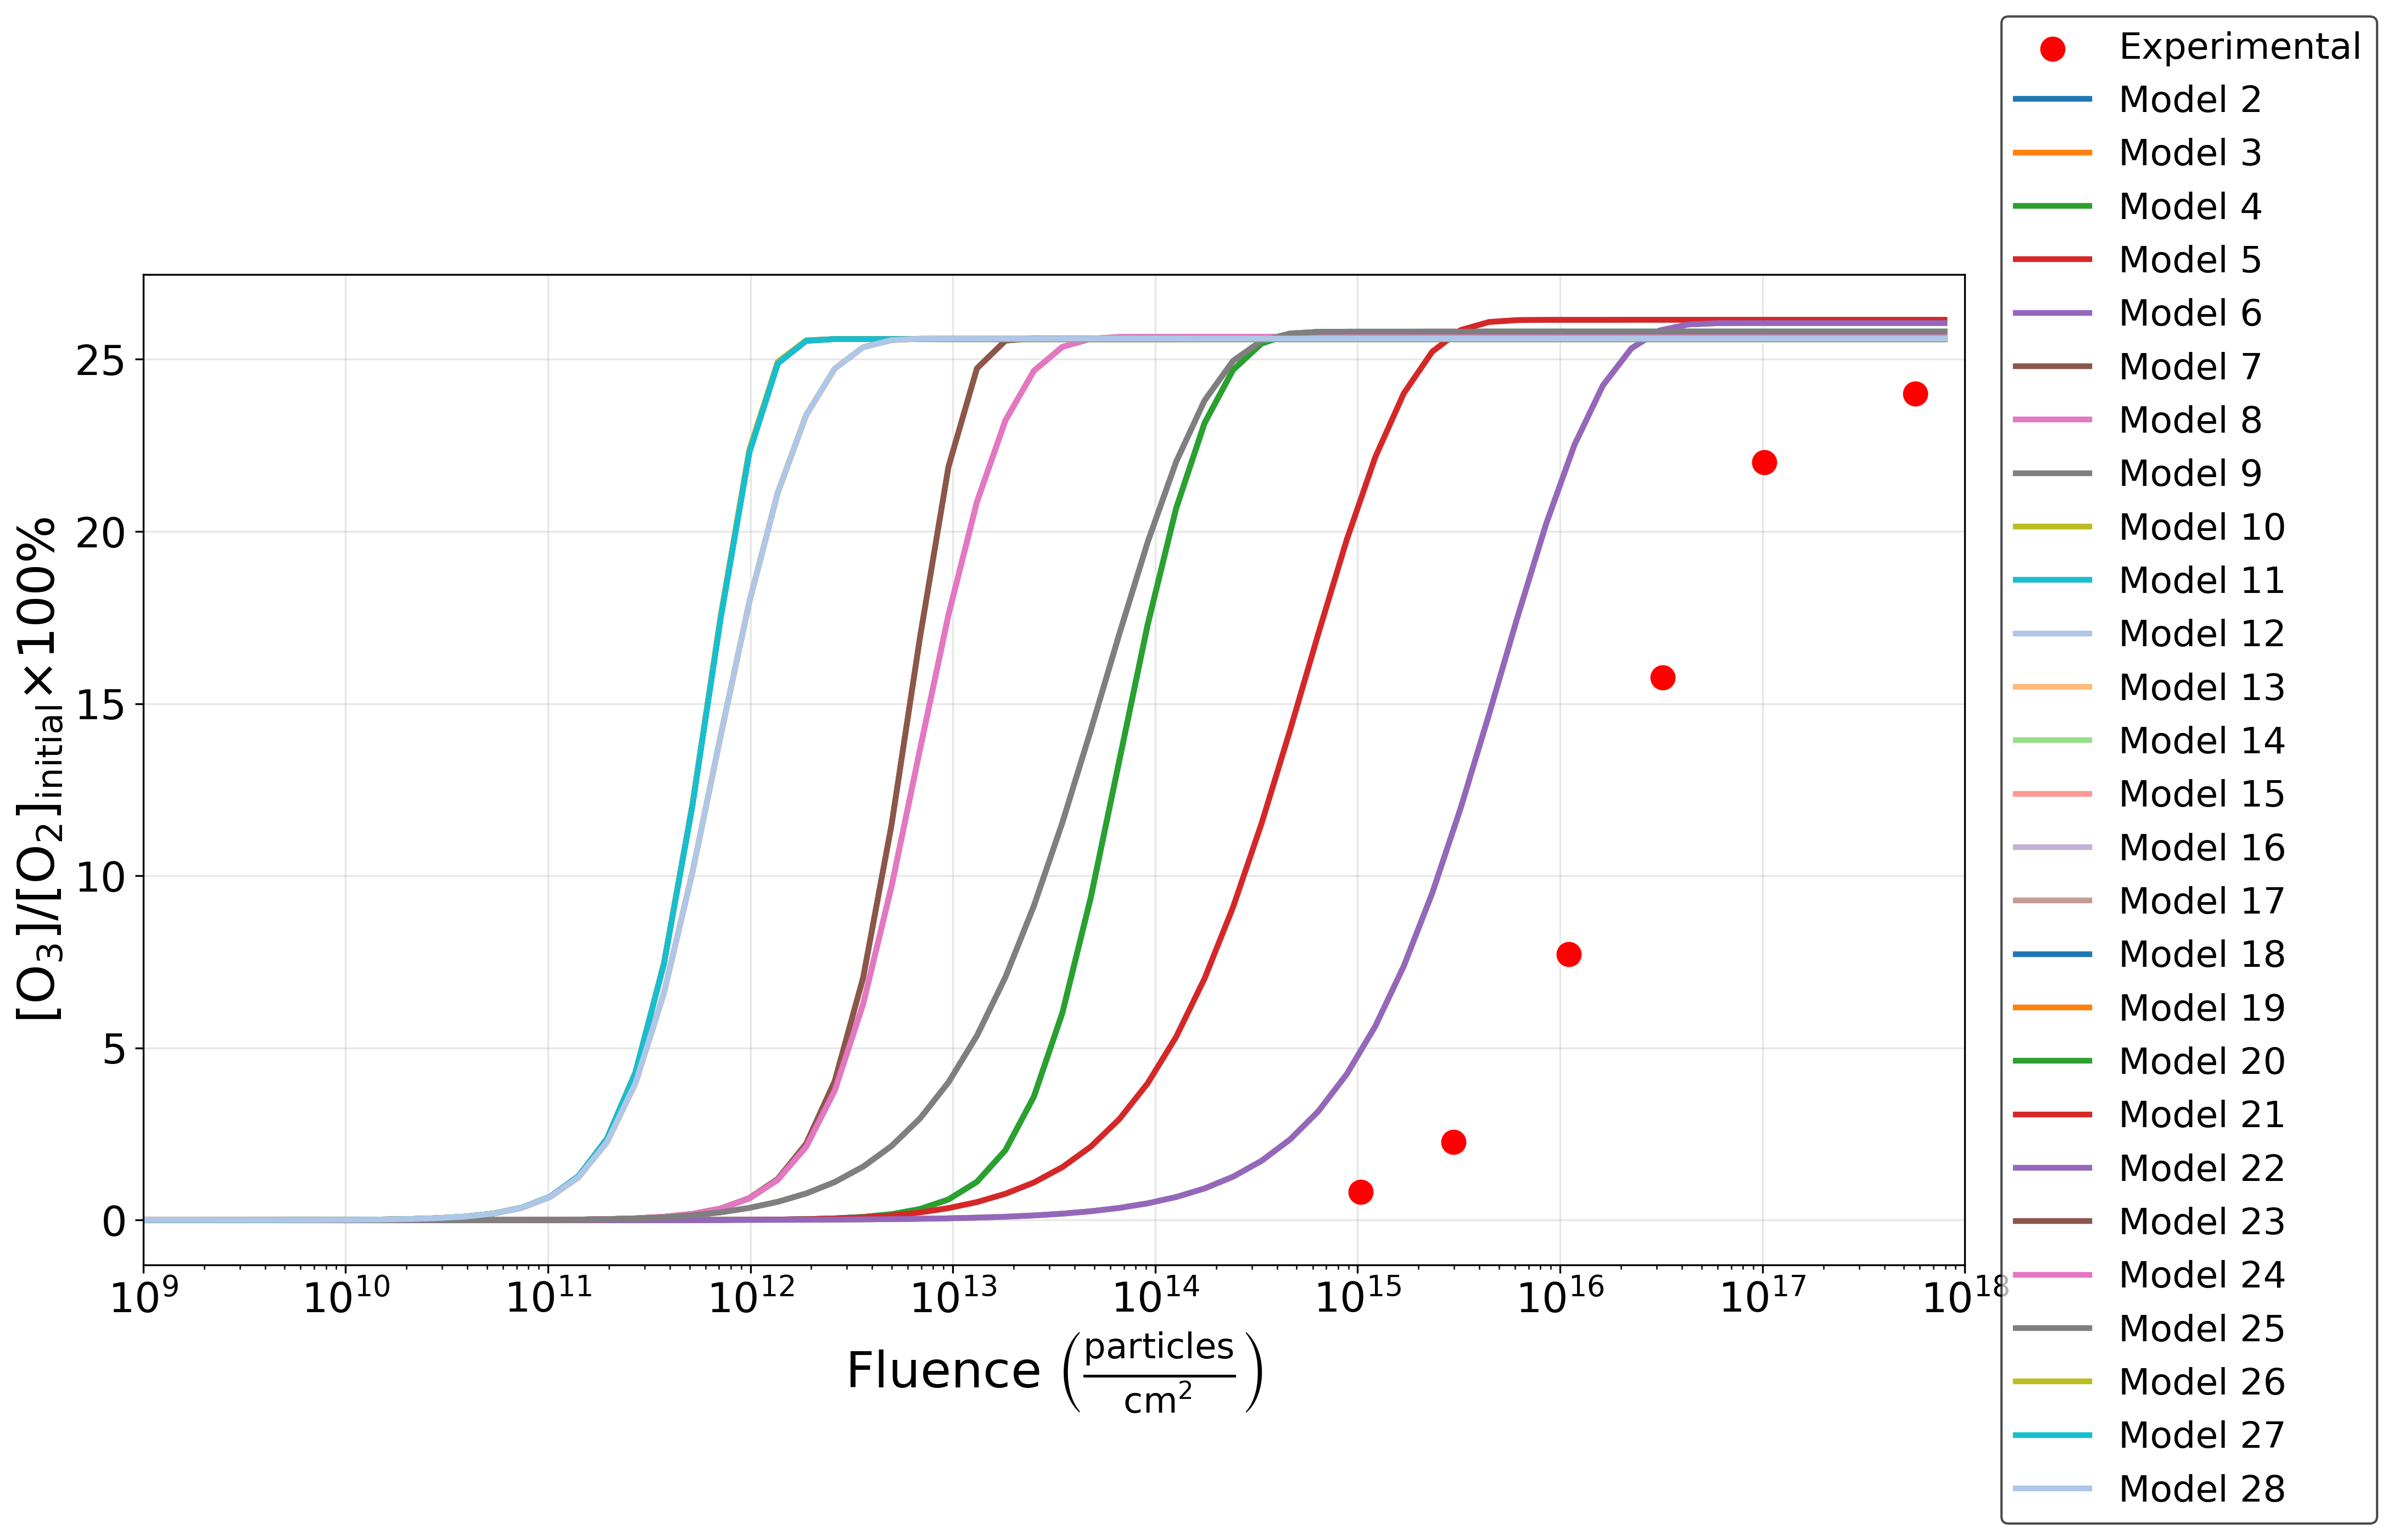
\includegraphics[width=0.9\linewidth]{f2.png}
    \caption{Models 2-28 (solid lines) compared with experimental data (points).}
    \label{fig:othermodels}
\end{figure*}

\subsection{\cb{Same-Model Ion-Off Control}}

\cb{To directly assess the role of ionic channels in Model 1, we also carried out a same-model ion-off control in which only the photoprocess channels yielding charged products were suppressed, while all neutral channels, trial frequencies, and all other Model 1 settings were held fixed. This is a cleaner diagnostic than reverting to an earlier ion-free network because it isolates the ionic contribution within the present model framework. In this control, the agreement with the \citet{gerakines_ultraviolet_1996} \ce{O3} data deteriorates markedly: the unweighted root-mean-square deviation $\chi$ increases from 0.484 in the full ion-enabled Model~1 to 13.93 in the ion-off case, and the peak modeled \ce{O3} abundance falls from 23.5\% to 3.24\% of the initial \ce{O2}. The ion-on and ion-off trajectories are compared directly in Fig.~\ref{fig:ionoff_overlay}. Thus, neutral chemistry alone can still produce some ozone, but is quantitatively insufficient within the present Model~1 network to reproduce the observed abundance trajectory; the ionic channels are not a minor refinement of an otherwise sufficient neutral model, but provide kinetically important pathways required to recover both the magnitude and fluence dependence of the measured \ce{O3} growth.}

\begin{figure}[htb]
    \centering
    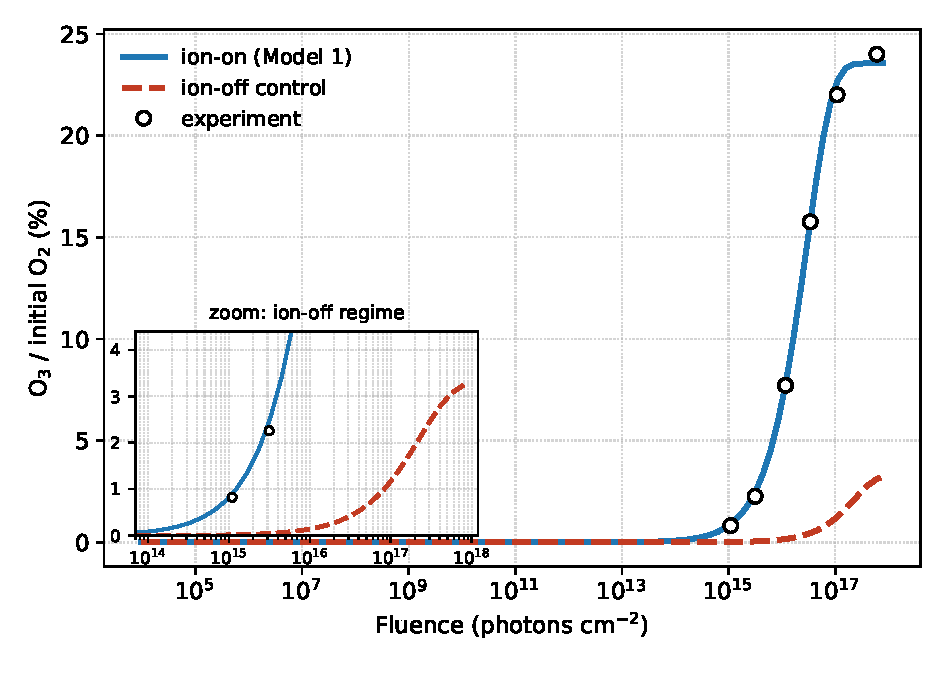
\includegraphics[width=\columnwidth]{f7.pdf}
    \caption{\cb{Same-model ion-on / ion-off comparison for Model~1. The solid curve shows the ion-enabled baseline, the dashed curve the control in which only charged-product photoprocess channels are suppressed, and the symbols the experimental points from \citet{gerakines_ultraviolet_1996}. Muting the charged-product channels degrades the fit from $\chi = 0.484$ to $\chi = 13.93$ and lowers the peak modeled \ce{O3} abundance from 23.5\% to 3.24\% of the initial \ce{O2}.}}
    \label{fig:ionoff_overlay}
\end{figure}

\subsection{Neutral Species}

\begin{table*}[p!]
  \caption{Delta value for photoprocesses in Model 1}
  \label{tbl:best_params}
 \begin{tabular}{l l c c l  c }
 \hline
 Number & Type &  & Process &  & $\delta$\\ 
 \hline
 %R1 Ionization Processes
 \ref{plabel1} &   R1  & \ce{O}  & $\leadsto$ & \ce{O+} + \ce{e-}    & $1.00$  \\
 \ref{plabel2} &   R1  & \ce{O2} & $\leadsto$ & \ce{O+} + \ce{O-}    & $0.437$  \\
 \ref{plabel3} &   R1  & \ce{O2} & $\leadsto$ & \ce{O2+} + \ce{e-}   & $1.54$  \\
 \ref{plabel4} &   R1  & \ce{O3} & $\leadsto$ & \ce{O+} + \ce{O2-}   & $1.00$  \\
 \ref{plabel5} &   R1 & \ce{O3} & $\leadsto$  & \ce{O2+} + \ce{O-}   & $1.00$  \\
 \ref{plabel6} &   R1 & \ce{O3} & $\leadsto$  & \ce{O3+} + \ce{e-}   & $1.00$  \\
 %R2 Ionization Processes
 \ref{plabel7} &   R2  & \ce{O} & $\leadsto$  & \ce{O^*}             & $1.00$  \\
 \ref{plabel8} &   R2  & \ce{O2} & $\leadsto$ & \ce{O^*} + \ce{O^*}  & $1.90$ \\
 \ref{plabel9} &   R2  & \ce{O3} & $\leadsto$ & \ce{O2^*} + \ce{O^*} & $1.00$  \\
 %R3 Excitation Processes
 \ref{plabel10} &   R3 & \ce{O} & $\leadsto$   & \ce{O^*}             & $1.00$  \\
 \ref{plabel11} &   R3 & \ce{O2} & $\leadsto$  & \ce{O2^*}            & $99.0$  \\
 \ref{plabel12} &   R3 & \ce{O3} & $\leadsto$  & \ce{O3^*}            & $99.0$  \\
 %R4 Excitation Processes
 \ref{plabel13} &   R4 & \ce{O2} & $\leadsto$  & \ce{O} + \ce{O}      & $1.00$  \\
 \ref{plabel14} &   R4 & \ce{O3} & $\leadsto$  & \ce{O2} + \ce{O}     & $22.1$  \\
 \hline
 \end{tabular}
\end{table*}

\begin{figure*}[!p]
\centering
\subfloat[\ce{O3}\label{fig:othreerxn}]{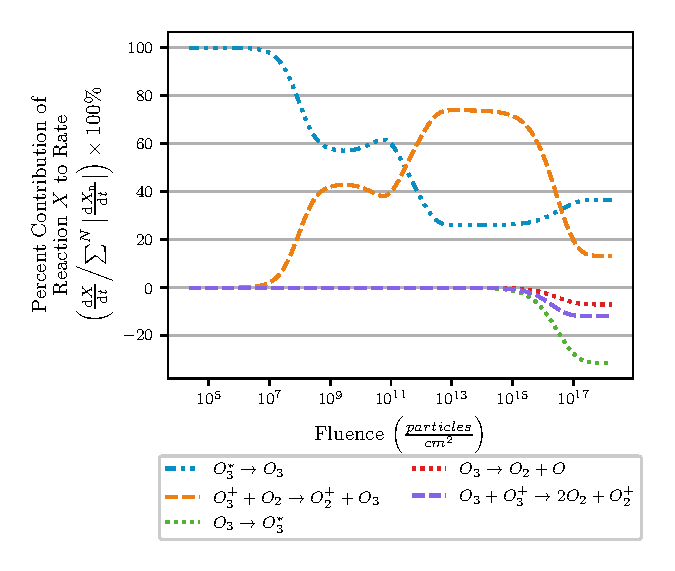
\includegraphics[width=0.45\linewidth]{f3a.eps}}\hfill
\subfloat[\ce{O3}$^*$\label{fig:othreesuprarxn}]{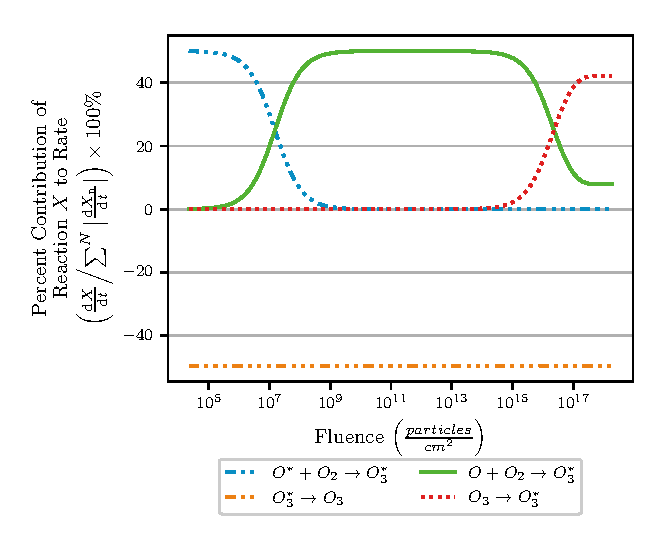
\includegraphics[width=0.45\linewidth]{f3b.eps}}\\
\subfloat[\ce{O}\label{fig:orxn}]{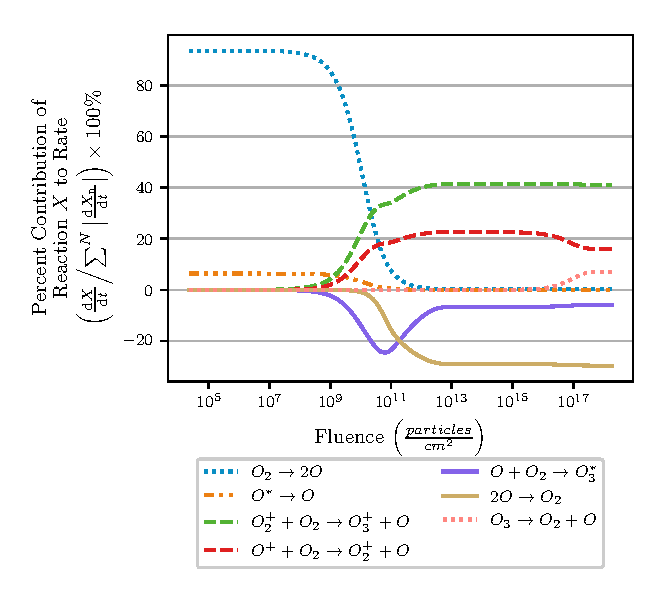
\includegraphics[width=0.45\linewidth]{f3c.eps}}\hfill
\subfloat[\ce{O}$^*$\label{fig:osuprarxn}]{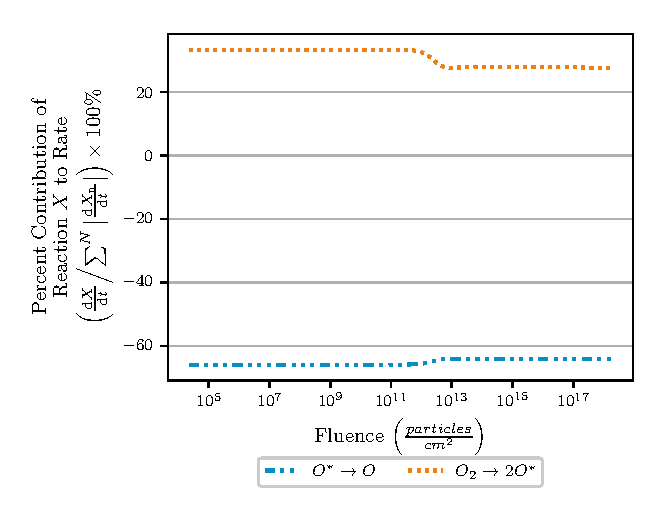
\includegraphics[width=0.45\linewidth]{f3d.eps}}\\
\subfloat[\ce{O2}\label{fig:otworxn}]{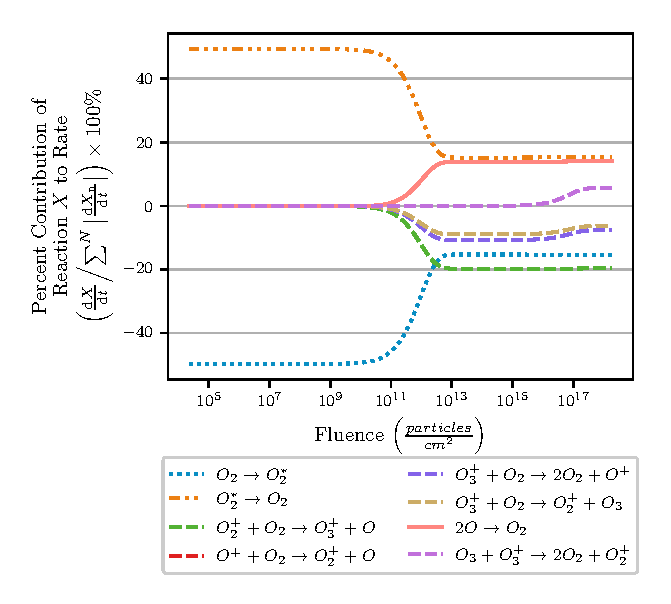
\includegraphics[width=0.45\linewidth]{f3e.eps}}\hfill
\subfloat[\ce{O2}$^*$\label{fig:otwosuprarxn}]{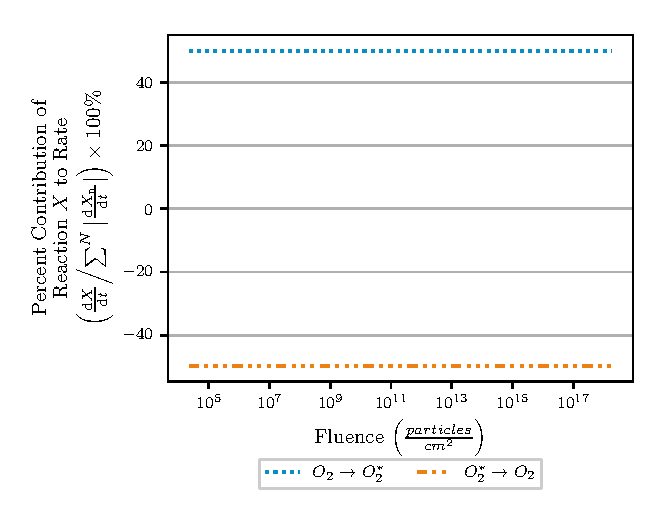
\includegraphics[width=0.45\linewidth]{f3f.eps}}
\caption{Relative importance of formation and destruction reactions for neutral species and their suprathermal counterparts in Model 1. See Table \ref{tbl:legend} for an explanation of the different linestyles.}
\label{fig:grid}
\end{figure*}

In this section, we detail the chemistry of the neutral species in our chemical network (O, \ce{O2}, and \ce{O3}), as well as of their suprathermal counterparts. Each of their major formation and destruction reactions is shown in Fig. \ref{fig:grid}. We note that Table \ref{tbl:legend} describes the meaning of the different line styles in the reaction contribution figures presented here. 

\begin{table}
        \footnotesize
      \caption{Line styles in Reaction Contribution Plots}
      \label{tbl:legend}
      \begin{tabular}{clc}
        \hline
        Line Style & Reaction Category   \\                
        \hline
        \tikzSolidLine & neutral-neutral reactions \\
        \tikzDashedLine & ion-neutral reactions \\
        \tikzDashDottedLine & ion-recombination reactions \\
        \tikzDottedLine & photoprocesses \\
        \tikzDashThreeDottedLine & suprathermal/quenching reactions \\
        \hline 
      \end{tabular}
      %Definitions for tikz lines are located in tikz_defs.tex
\end{table}

\subsubsection{\ce{O3} and \ce{O3}$^*$}

As shown in Fig. \ref{fig:othreerxn}, the chemistry of ozone largely follows what was found previously in Mullikin et al. \citep{mullikin_new_2021} at early and late fluences. Here, as there, the dominant formation route for ozone is the two-step process

\begin{equation}
    \ce{O} + \ce{O2} \rightarrow{} \ce{O3^*} \leadsto{} \ce{O3}
    \label{ozoneneutralformation}
\end{equation}

\noindent
where suprathermal \ce{O3^*} is first formed from the reaction of ground state atomic and molecular oxygen, or between suprathermal oxygen and ground state molecular oxygen. In both cases, suprathermal ozone is destroyed via quenching by the bulk ice (See Figure \ref{fig:othreesuprarxn}).

Conversely, at intermediate fluences, the underlying chemistry of \ce{O3} in the model changes dramatically, highlighting the potentially critical role of ions for understanding the chemistry of irradiated low-temperature solids, with the dominant formation pathway ($\sim70$\%) becoming

\begin{equation}
    \ce{O3+ + O2 -> O2+ + O3}.
    \tag{\ref{nlabel35}}
\end{equation}

In Model 1, ozone is destroyed mainly by either photolysis or reaction with \ce{O3+}, again highlighting the potential importance of ions in bulk chemistry. 


\subsubsection{\ce{O} and O$^*$}


As can be seen in Fig. \ref{fig:orxn}, the chemistry of atomic oxygen largely follows a similar pattern as \ce{O3}. At early fluences, neutral chemistry dominates, with the main formation route being

\begin{equation}
    \ce{O2 \leadsto{} 2O}
    \tag{\ref{plabel13}}
    \label{oformation}
\end{equation}

\noindent
and the major destruction pathways being the reformation of molecular oxygen

\begin{equation}
    \ce{O + O -> O2}
    \label{odestruction}
\end{equation}

\noindent
or reaction with \ce{O2} to form suprathermal ozone.

However, as with \ce{O3}, ion-neutral reactions become more important at later fluences, as depicted in Fig. \ref{fig:orxn}. After a fluence of $10^{11}$ photons cm$^{-2}$ is reached, the reactions

\begin{equation}
    \ce{O2+ + O2 -> O3+ + O}
    \tag{\ref{nlabel20}}
    \label{otwoiondest}
\end{equation}

\noindent
and

\begin{equation}
    \ce{O+ + O2 -> O2+ + O}
    \tag{\ref{nlabel9}}
\end{equation}

\noindent
become more significant, representing roughly 40\% and 20\% of the O formation, respectively. 

For the case of suprathermal oxygen, depicted in Fig. \ref{fig:osuprarxn}, the situation is quite simple. At all fluences, it is mainly formed via 

\begin{equation}
    \ce{O2} \leadsto 2\ce{O}^*.
    \tag{\ref{plabel8}}
\end{equation}

\noindent
Similarly, the major destruction pathway throughout the model is quenching by the ice.

\subsubsection{\ce{O2} and \ce{O2}$^*$}

For \ce{O2} reactions, represented in Fig. \ref{fig:otworxn}, the dominant formation route at early fluences (before $\sim10^{12}$ cm$^{-2}$) comes simply from the quenching of suprathermal \ce{O2}. After that time, the bimolecular reaction between ground-state oxygen atoms becomes more important. Destruction is initially dominated by electronic excitation leading to suprathermal molecular oxygen. After $\sim10^{12}$ cm$^{-2}$, ion-neutral destruction routes become more important, including the reaction of molecular oxygen with \ce{O2+} (\ref{nlabel20}), as well as the reactions

\begin{equation}
    \ce{O3+ + O2 -> O2+ + O3}.
    \tag{\cb{\ref{nlabel35}}}
\end{equation}

\noindent
and

\begin{equation}
    \ce{O3+ + O2 -> 2O2 + O+},
    \tag{\ref{nlabel37}}
\end{equation}
 
For suprathermal molecular oxygen, shown in Fig. \ref{fig:otwosuprarxn}, at all model times the dominant formation route is via the excitation process \ref{plabel11}. Similar to the other suprathermal species, the dominant destruction pathway is via quenching.

\FloatBarrier
\subsection{Ions}\label{sec:ionchemistry}

\begin{figure}[htb]
    \centering
    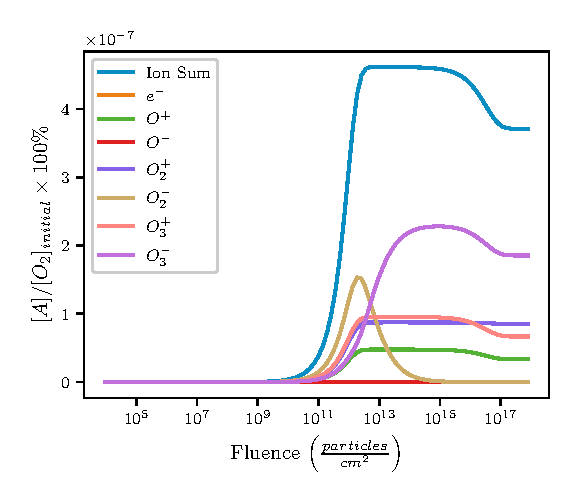
\includegraphics[width=\columnwidth]{f4.eps}
     \caption{Total abundance of solid-phase ions vs. fluence.}
     \label{fig:ionabundance}
\end{figure}%

Fig. \ref{fig:ionabundance} shows the calculated abundances of the cations and anions in our simulation as a function of fluence. There, one can see that the combined peak abundance of all charged species remains very low, with a value of $\sim1.2\times10^{-6}$\% by the end of the simulation. Here, we describe the main formation and destruction pathways of key ionic species.

\begin{figure*}[!tb]
\centering
\subfloat[\ce{O2-}\label{fig:otwominusrxn}]{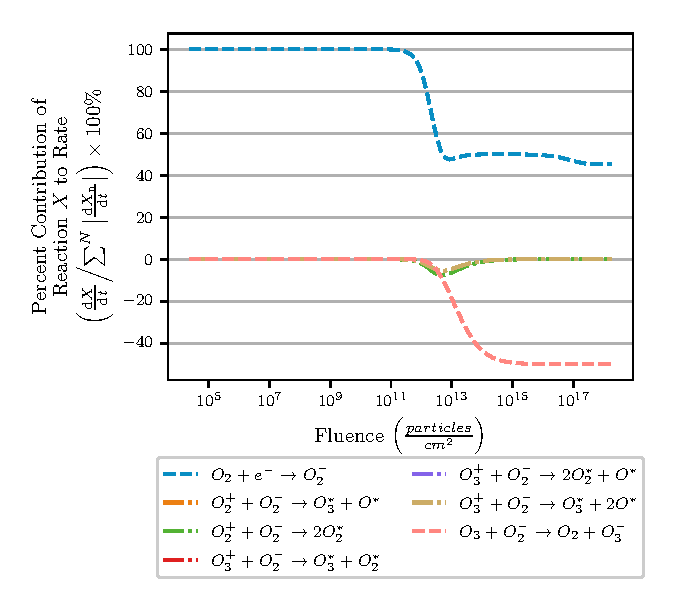
\includegraphics[width=0.45\linewidth]{f5a.eps}}\hfill
\subfloat[\ce{O3-}\label{fig:othreeminusrxn}]{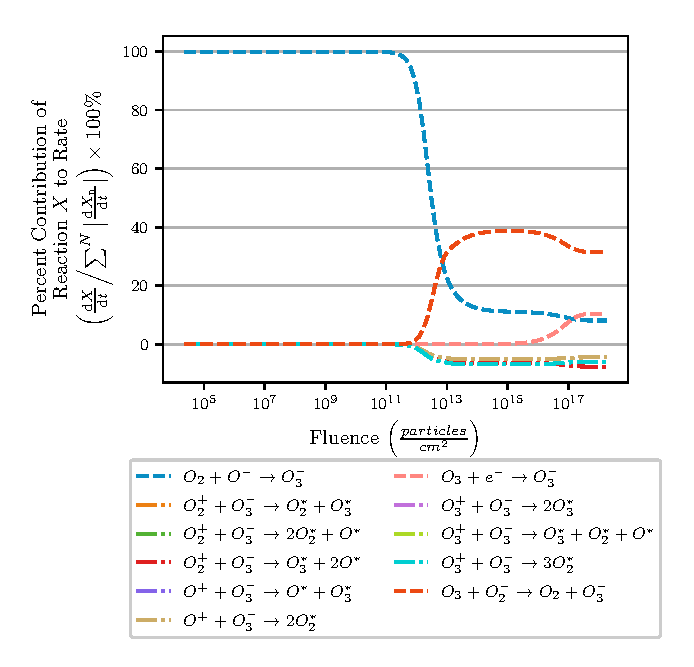
\includegraphics[width=0.45\linewidth]{f5b.eps}}
\caption{Relative importance of formation and destruction reactions for (a) \ce{O2-} and (b) \ce{O3-} in Model 1. See Table \ref{tbl:legend} for an explanation of the different linestyles.}
\label{fig:ions}
\end{figure*}

Before a fluence of $\sim10^{11}$ cm$^{-2}$, the abundance of ions is quite low. Afterwards, however, there is a noticeable increase in their abundance, with \ce{O2-} being initially the most abundant. As depicted in Fig. \ref{fig:otwominusrxn}, this anion is formed at all model times mainly via the associative attachment of an electron

\begin{equation}
    \ce{O2 + e- -> O2-}
    \tag{\ref{nlabel14}}
\end{equation}

\noindent
and is destroyed via a number of reactions, with the most important after $\sim10^{13}$ cm$^{-2}$ being the charge transfer reaction

\begin{equation}
    \ce{O3 + O2- -> O2 + O3-}.
    \tag{\ref{nlabel28}}
\end{equation}

After a fluence of $\sim10^{14}$ cm$^{-2}$, \ce{O3-} becomes the dominant charged species in Model 1. As shown in Fig. \ref{fig:othreeminusrxn}, it is initially formed mainly via 

\begin{equation}
    \ce{O2 + O- \rightarrow{} O3-}
    \tag{\ref{nlabel15}}
\end{equation} 

\noindent
with the reaction 

\begin{equation}
    \ce{O3 + O2- -> O3- + O2}
    \tag{\ref{nlabel28}}
\end{equation}

\noindent
becoming important at later fluences. The destruction of \ce{O3-} occurs entirely through ion-recombination reactions. We note that the plots of the eight ion-recombination reactions obscure each other in Fig. \ref{fig:othreeminusrxn}.

\subsubsection{Electrons}

Finally, the addition of electrons in our network is another novel feature and a byproduct of the ionizing radiation that real astrophysical ices are continuously exposed to. As shown in Fig. \ref{fig:erxn}, electron chemistry is dominated by the ionization and subsequent recombination with the dominant ice constituents. Specifically, they are produced overwhelmingly from the photoionization of \ce{O2} and destroyed via recombination with \ce{O2} and \ce{O3}. We note that in these preliminary simulations, we have not included processes which are critical for very low energy ($<$ 5 eV) electrons, such as dissociative electron attachment (DEA), though such processes undoubtedly occur in real irradiated ices \citep{arumainayagam_low-energy_2010}. Future simulations will examine the effects of low-energy electrons in more detail.


\begin{figure}[htb]
    \centering
    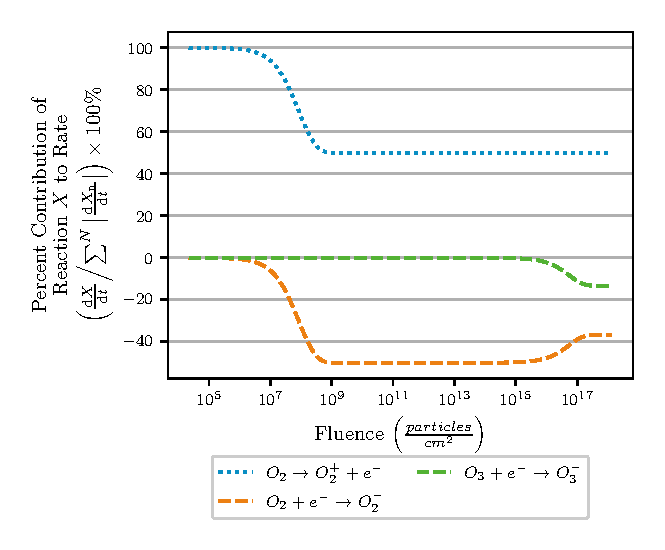
\includegraphics[width=\columnwidth]{f6.eps}
    \caption{Major reactions with electrons.}
    \label{fig:erxn}
\end{figure}%
           
\section{Conclusions} \label{sec:conclusions}

In this work, we describe novel astrochemical simulations which seek to elucidate the effects of solid-phase ions on the chemistry of low-temperature solids, specifically, within interstellar dust grain ice mantles. Expanding on our previous models described in \citet{shingledecker_simulating_2019} and \citet{mullikin_new_2021}, we have used the method of \citet{shingledecker_general_2018} to model the production of ionic species formed from the photoionization and photoexcitation of atoms and molecules within the ice. To examine the effects of such ions on solid-phase chemistry under well-constrained conditions, we carried out simulations of pure \ce{O2} ice at 10 K irradiated by UV photons, following the work of \citet{gerakines_ultraviolet_1996}, who tracked the production of ozone under those conditions.

The models described here show that inclusion of ionic species and related reactions is possible in three-phase, slightly modified astrochemical codes, with the caveat that such additions do substantially increase the size, complexity, and uncertainty of the chemical networks. \cb{Our results further indicate that ionic pathways are kinetically important for reproducing the observed \ce{O3} growth in Model~1. Although neutral channels dominate several gross terminal \ce{O3}-forming steps, particularly at early and late fluence, ion-neutral and ion-ion processes govern the mid-fluence chemistry and materially improve agreement with experiment. The stronger sensitivity of the calculated abundances to $\nu_\mathrm{i-n}$ and $\nu_\mathrm{i-i}$ than to $\nu_\mathrm{n-n}$ further suggests that the ionic sector regulates the precursor supply, recycling, and destruction balance feeding those neutral terminal steps, even when the dominant terminal formation routes themselves remain neutral. In this sense, the explicit inclusion of ion-neutral and ion-ion chemistry is not simply an optional refinement of the neutral backbone developed in our previous work \citep{mullikin_condensed-phase_2018,shingledecker_simulating_2019}, but a load-bearing component of the kinetics required to recover the observed \ce{O3} abundance trajectory in the present model family.}

Future studies using this method could fruitfully be applied to studying systems where solid-phase ion-neutral and ion-ion reactions are likely to play a larger role, such as those involving the formation of salts or the kinds of charged species which have been detected in cometary material \citep{altwegg_evidence_2020} and real interstellar dust-grain ice mantles \citep{mcclure_ice_2023,yang_corinos_2022}. Overall, though, the results of our calculations are in line with other recent studies, notably by \citet{woon_ion-ice_2011} and \citet{woon_formation_2024} who studied bulk-ice chemistry, and both \citet{nakai_methanol_2023} and \citet{cui_exploring_2024}, who studied surface processes, in showing that, as is the case with gas-phase processes, the reactions of charged species on interstellar dust grains likely represent an important class of chemical processes that will need to be examined in more detail in the future. Of particular utility for future modeling studies would be experimental data on the fluence-dependent abundance of multiple components of an ice-analogue, as well as information about the total concentration and makeup of ions in-situ in the ice. 


%%%%%%%%%%%%%%%%%%%%%%%%%%%%%%%%%%%%%%%%%%%%%%%%%%%%%%%%%%%%%%%%%%%%%
%% The "Acknowledgement" section can be given in all manuscript
%% classes.  This should be given within the "acknowledgement"
%% environment, which will make the correct section or running title.
%%%%%%%%%%%%%%%%%%%%%%%%%%%%%%%%%%%%%%%%%%%%%%%%%%%%%%%%%%%%%%%%%%%%%
\begin{acknowledgement}
L.M. acknowledges financial support from DAE and DST-SERB research grant (MTR/2021/000864) from the Government of India for this work. 


\end{acknowledgement}

%%%%%%%%%%%%%%%%%%%%%%%%%%%%%%%%%%%%%%%%%%%%%%%%%%%%%%%%%%%%%%%%%%%%%
%% The same is true for Supporting Information, which should use the
%% suppinfo environment.
%%%%%%%%%%%%%%%%%%%%%%%%%%%%%%%%%%%%%%%%%%%%%%%%%%%%%%%%%%%%%%%%%%%%%

%%%%%%%%%%%%%%%%%%%%%%%%%%%%%%%%%%%%%%%%%%%%%%%%%%%%%%%%%%%%%%%%%%%%%
%% The appropriate \bibliography command should be placed here.
%% Notice that the class file automatically sets \bibliographystyle
%% and also names the section correctly.
%%%%%%%%%%%%%%%%%%%%%%%%%%%%%%%%%%%%%%%%%%%%%%%%%%%%%%%%%%%%%%%%%%%%%
\bibliography{references}

\end{document}
